\section{Considerations for Dataset Selection}\label{sec:cheminf}

Despite the vast amount of literature published in chemistry, there are surprisingly only a limited number of datasets available to the public. There are many considerations that must be made for selecting a dataset, and in many cases cleaning a dataset for use in machine learning. I will discuss some considerations when selecting and using a new dataset of molecules.

First, it is important to consider what kind of data is contained in the dataset. Are values predicted values, or values from an electronic structure calculation or another kind of calculation. Models trained on datasets containing calculated values alone can only be used to predict other calculated properties. If one desires to use the model to predict a measured property, then it is necessary to either use a transfer learning approach, or otherwise calibrate the measured properties to calculated data.

Second, one must consider the size of the dataset. Many datasets which contain measured properties typically only contain properties for a few hundred molecules at best. On such a small dataset, it becomes easy to overfit the model. While it would be possible to develop a model for predicting this dataset, it may not be very generalizable to other datasets.

A related, important factor to consider is the diversity of molecules in the dataset. Are there only a few families of molecules represented? Are some families of molecules more heavily represented than others? Machine learning models are excellent interpolation models, but cannot extrapolate to examples it has not seen before. In other words, a model that has been trained on only one or two families of molecules may would be excellent at predicting properties for molecules in these families, but likely unable to predict properties for molecules outside of this family.

A few large datasets of molecules exist, some with some predicted properties. A more extensive list is provided in these reviews. Some of the datasets used in these thesis include:
\begin{itemize}
\item \textbf{QM9} : A dataset for molecules with fewer than 9 heavy (non-hydrogen) atoms, containing calculated properties
\item \textbf{ZINC} : A dataset of drug molecules. The entire dataset contains millions of molecules, but these can be filtered down to a smaller group.
\item \textbf{NIST 17 Mass Spectral Library}: This collection of data is not available to the public, but is accessible to researchers whose institutions have access to mass spectral software.
\end{itemize}

Once a dataset has been settled upon, typically it is necessary to clean the dataset. Cleaning the dataset can take on a whole range of tasks. A typical workflow to prepare a new dataset is as follows:
Write a parser to convert the molecule data file into a format readable for machine learning tasks.
Using database visualization tools, examine the dataset for any errors. In particular, pay attention to any outliers in the dataset, or any values that are unphysical (e.g. a molecule containing a mass spec intensity peak at an m/z ratio that is much larger than the mass of the molecule itself).
Create a linear regression model or a single layer model for predicting the output to ensure that everything runs correctly.

Inevitably, for each dataset which contains new properties, it will be necessary to add a few extra data parsing steps, or add a few more sanity checks into the data processing pipeline. Visualizing the data and the predictions as often as possible is the key to identifying potential errors in the dataset.

\section{Molecule Descriptors}

Machine learning models require vectorized information as inputs to the model. The matrix multiplication operations which underpin the layers of a machine learning model will transform these input vectors into new features or predictions.

For many problems in machine learning, such as vision recognition, vectorizing inputs is straightforward. Images are composed of pixels, with an RGB value or greyscale associated with each pixel, and so these data inputs are already in vectorized form. Converting molecules into a vector representation is not simple.

One can think of a molecule as a graph, with the atoms as nodes and the bonds between the atoms as edges. What is the best way to vectorize information from a graph? This depends on what one wants to learn from the model. For example, if one simply wanted to 'learn' the molecular weight given a molecule, then a vector representation that includes all the atoms is sufficient.

If one wanted to optimize for something more complicated, such as which molecule might be suitable for  flow battery applications, then some of the properties one would want the model to predict include: the reduction potential, the susceptibility of the molecule to reactions with water and other molecules in the environment\cite{tabor_2018}.

To understand what features we'd like to incorporate into our vector representation of a molecule in order to predict these properties, let's consider what properties a human organic chemist would observe in the molecule. Looking at the molecule, a chemist might have an idea of these properties by examining:

The number of rings contained in a molecule, or the overall stability of the molecule
The types of subgroups that are bound to the ring. In particular, are these fragments electron withdrawing or electron donating?
How many such groups are bound to the molecule?
Which positions are electron donating and accepting? How accessible are these positions to other molecules.

All of these aspects of a molecule cannot be captured by simple atom-level descriptors. Instead it is necessary for descriptors to consider neighborhoods around atoms.

I will now describe some existing molecule representation methods.

\subsection{Descriptors from Cheminformatics}

Since the 1960s, chemists have leveraged computable information on molecules towards predicting properties in drug discovery. This discipline is known as cheminformatics; numerous books and reviews have been written about this topic\cite{gasteiger2014solved,chonde2014cheminformatics,warr2005twenty,gasteiger2015cheminformatics}.

The key goal of cheminformatics is to identify quantitative structure property relationships (QSAR); these relationships are based on the notion that the functionality of a molecule for any particular application is defined by its structure. As such, by analyzing the structure, either by using quantum mechanics modeling techniques, or some other data-driven methods, it is possible to determine the molecule's usefulness for the application. In turn, it is possible to use these patterns to identify promising candidates for a given application.

The earliest machine-readable representations of molecules were developed from this field. Most of these descriptors are in the form of some sort of string descriptor. In present research, the most popular string representations include the SMILES (Simplified Molecular Input Line Entry Specification) and the INCHI (IUPAC International Chemical Identifier) representations\cite{weininger1988smiles}.  Both SMILES strings and INCHI representation encode not only the atoms present in the molecule, but also the connections between the atoms in the molecule. Figure \ref{fig:molecule_reps} has an example of a molecule encoded in SMILES representation, the different colors in the string representing different parts in the molecule. The INCHI representation also contains additional information about stereochemistry. A hashed version of the INCHI, known as the INCHIKEY is a common molecule identifier. The SMILES representation is used heavily in Chapter 4 of this work.

Various descriptors can be derived based on these raw representations; in fact, there are several software packages which provide hundreds of these descriptors for users\cite{rdkit,mauri2006dragon}. These properties describe the partial charge of the molecule, the solvent accessible area, etc. Many of these properties can be calculated using heuristic models, e.g. Gasteiger charges. These descriptors can in turn be used to model more complicated properties that are more pertinent to the problem that one wishes to optimize\cite{mauri2006dragon}.

A more abstract molecule descriptor is the family of fingerprint descriptors. Fingerprints capture local information about the molecule's structure and encode this information in a vector. The type of local information varies for each fingerprint.

Morgan fingerprints/Extended Circular Fingerprints \cite{morgan1965generation,Rogers_2010_ECFP} capture the local environment around each atom, as shown in Figure\ref{fig:molecule_reps}. This information records all local neighborhoods of molecule fragments which contain fewer than the maximum bond radius to consider. In order to generate a fixed length vector representation, the information about the local structure is hashed into a vector. Chapters 3 and 5 of this thesis feature applications of this fingerprint.

\begin{figure}
\begin{center}
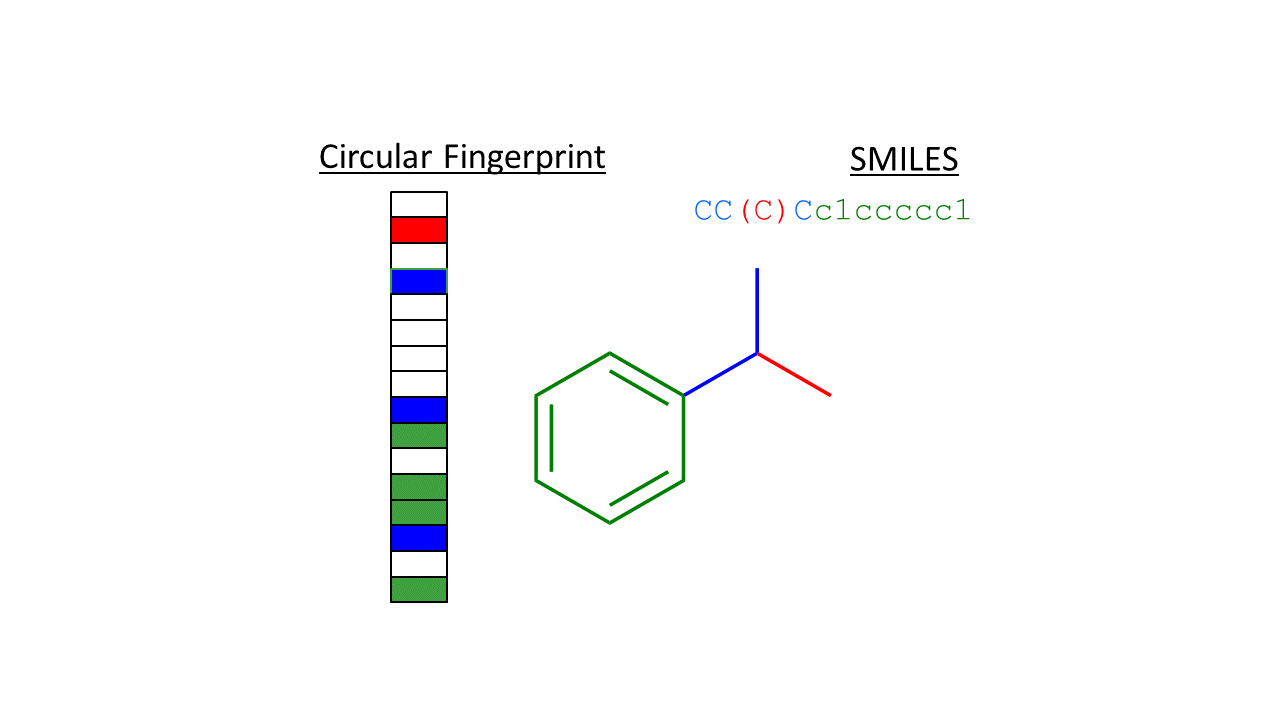
\includegraphics[width=0.9\columnwidth]{molecule_reps.png}
\caption[SMILES and Circular Fingerprint Molecular Representation]{
SMILES and Circular Fingerprints. Color coding is added as a visual aid, colored portions of
the representation correspond to different parts of the representation.
In the SMILES representation, a string is used to represent the molecular graph.
Branching regions are encoded in parenthesis (red) while cycles are encoded by starting and ending
the cyclical region with a number (green). Lower case letters are used to represent atoms which
are in an aromatic ring (green). The Circular fingerprint is a binary vector representation of a
molecule. Molecular subgraphs centered around different atoms are recorded as bits in the fingerprint.
}
\label{fig:molecule_reps}
\end{center}
\end{figure}


Other fingerprints vary in their focus on known functional groups within the molecule (e.g. MACCS Fingerprint)\cite{durant2002reoptimization} or their focus on three dimensional structure (e.g. Topological fingerprints)\cite{nilakantan1987topological}. The precise fingerprint, or combination of fingerprints to use often depends on the application at hand. It is often useful to test multiple fingerprints, or even combinations of fingerprints, to determine which might be the best for representing molecules for the given application\cite{kim2017multidk}.


\subsection{Chemical Graph theory}

The subfield of chemical graph theory considers graph-theory based approaches to molecule representations\cite{randic2016solved}. These representations typically describe the whole molecule graph, rather than describing local fragments or representing some estimated physical properties.

Some of the more common descriptors from this field include the adjacency matrix and the Coulomb matrix\cite{rupp2012fast}. Other descriptors include the eigenvalues of the adjacency matrix, path indices, and topological indices. Path indices describe the longest path between two carbon atoms present in a molecule\cite{randic2016solved}.
Topological indices depend on the valences of the constituent atoms in a bond\cite{randic2016solved}.

Descriptors from this field are used less often, they do not enjoy the same level of support in open source packages as the cheminformatic descriptors. Descriptors from this field have been used to predict a wide variety of properties, including the boiling points for alkane, amino alkenes, predicting antihypertensive activity, and NMR shifts\cite{randic2016solved}.

\subsection{Descriptors developed with machine learning}

In the last two years, researchers have now applied machine learning to propose new molecular representations. Some of these representations extend the idea of the fingerprint representation as a two dimensional method for predicting molecules.
Known as graph convolutional networks\cite{duvenaud2015convolutional,kearnes2016molecular,gilmer_2017_mpnn}, these representations collect information from smaller subgraphs of the molecular graphs, and aggregate this information into a single vector.
The final output from these models is a continuous vector representation; this enables the parameters of the model itself to be tuned to predict a particular property.

New representations have also been developed for three dimensional molecule structures.  Starting with the three dimensional geometries allows for better prediction of some properties such as energies. In addition to graph convolutional models, wave transform models have been proposed for modeling the electron densities \cite{kuzminykh20183d}.
Wavelet scattering representations of the electron density have also been used as a rotationally invariant representation of a molecule\cite{eickenberg2017solid}.

\section{Afterword}

All of these descriptors have demonstrated their ability to predict energies/calculated properties for molecules. It is likely that using transfer learning techniques, it would be possible to use these models to model smaller experimental datasets.

However many of these machine learned representations proceeded the work in this thesis, or did not have an easily accessible implementation to use. As such, the work that is presented in the third part of this thesis uses two descriptors from cheminformatics: Morgan fingerprints and SMILES Representation.
